\documentclass[12pt, twoside]{article}
\usepackage[francais]{babel}
\usepackage[T1]{fontenc}
\usepackage[latin1]{inputenc}
\usepackage[left=1cm, right=1cm, top=1cm, bottom=2cm]{geometry}
\usepackage{float}
\usepackage{graphicx}
\usepackage{array}
\usepackage{multirow}
\usepackage{amsmath,amssymb,mathrsfs}
\usepackage{textcomp}


\begin{document} 

NOM: \\
PRENOM: 

\bigskip


\begin{center}
{\fbox{$2^{de}5$ \qquad \qquad \textbf{\Large{Devoir surveill� 3: 2h}}
\qquad \qquad 29/11/2008}}
\end{center}




\bigskip

\textit{Devoir � rendre sur feuille double petits carreaux. La clart� et la
pr�cision de la r�daction seront prises en compte.}

\bigskip



\fbox{\begin{minipage}{18cm}Les exercices 1, 2 et 3 sont � faire sur la feuille
photocopi�e. Pour ces 3 exercices, \textbf{la calculatrice n'est pas autoris�e}. Vous pourrez sortir
votre calculatrice \textbf{une fois cette feuille rendue.}
\end{minipage}}


\bigskip
\bigskip

\textbf{Exercice 1:} Simplifier au maximum l'�criture des nombres suivants (en
gardant les valeurs exactes):
\begin{enumerate}
  \item $|7-10|=$
  \item $|3-2\sqrt{2}|=$
  \item $|3 \pi -10|=$
  \item $\sqrt{(\sqrt{5}-3)^{2}}=$
  \item $|2 \sqrt{5}-\sqrt{21}|+|\sqrt{22}-\sqrt{20}|=$

\end{enumerate}

\bigskip

\bigskip

\textbf{Exercice 2:} Donner l'�criture scientifique des nombres suivants:
\begin{enumerate}
  \item $A=-0,000 \thinspace 352 \thinspace 148=$
  \item $B=4591,245=$
  \item $C=31,454 \times 10^{3}=$
  \item $D=245,12 \times 10^{-4}+0,000 \thinspace 184=$
\end{enumerate}

\bigskip

\bigskip

\textbf{Exercice 3:} \textit{Un peu de cours \ldots}
\begin{enumerate}
  \item Quelle est la valeur exacte de $\cos (45�)$?   \rule{3cm}{0,1mm}
 
 \item Qu'appelle-t'on m�diane dans un triangle? Quelles sont les propri�t�s
 associ�es � ces droites? 
 
 \rule{18cm}{0,1mm}
 
 \rule{18cm}{0,1mm}
 
 \rule{18cm}{0,1mm}
 
 \rule{18cm}{0,1mm}
 
 \rule{18cm}{0,1mm}
 
 \rule{18cm}{0,1mm}
 
 \item Quelle est la valeur exacte de la hauteur  d'un triangle �quilat�ral de
 c�t� $\sqrt{6}$?  \rule{3cm}{0,1mm}
 \item Sur la droite des r�els, soient $A$ le point d'abscisse $a$ et $B$ le
 point d'abscisse $b$. On appelle $I$ le milieu du segment $[AB]$. Quelle est
 l'abscisse du point $I$?  \rule{3cm}{0,1mm}
 \item Que signifie $|x|$?  
 
 \rule{18cm}{0,1mm}
\end{enumerate}

\pagebreak



\begin{center}
{\fbox{$2^{de}5$ \qquad \qquad \textbf{\Large{Devoir surveill� 3: 2h}}
\qquad \qquad 29/11/2008}}
\end{center}


\bigskip
\bigskip


\textbf{Exercice 4:} Pour chacun des cas suivants: repr�senter les intervalles
$I$ et $J$ sur une droite gradu�e et donner $I \cup J$ et $I \cap J$.
\begin{enumerate}
  \item $I=]-\infty;2]$ et $J=[1;3[$
  \item $I=[5;7]$ et $J=]6;7[$
  \item $I=[-4;-1[$ et $J=]0;1]$
\end{enumerate}

\bigskip

\textbf{Exercice 5:}
\begin{enumerate}
  \item Comparer $2+\sqrt{7}$ et $\sqrt{11+4 \sqrt{7}}$.
  \item Soient $x$ et $y$ deux r�els v�rifiant: $2 \leqslant x \leqslant 5$ et
  $1 \leqslant y \leqslant 4$. Donner un encadrement de $x^{2}-\dfrac{2}{y}$.
\end{enumerate}

\bigskip

\textbf{Exercice 6:} R�soudre les �quations et in�quations suivantes, justifier
vos r�sultats.
\begin{enumerate}
  \item $|x-8|=5$
  \item $|x-2|=|x+7|$
  \item $|x+1| \geqslant 2$
  \item $|x-6|<3$
\end{enumerate}

\bigskip

\textbf{Exercice 7:} Traduire � l'aide de valeurs absolues:
\begin{enumerate}
  \item $x \in [-1;3]$
  \item $x \in [5;8]$
  \item $x \in [\sqrt{2};\sqrt{3}]$
\end{enumerate}

\bigskip

\textbf{Exercice 8:} Pour chacune des propri�t�s (P1),(P2) et (P3): Enoncer la r�ciproque, dire si elle est vraie ou fausse.
  Dans le cas o� elle est fausse, donner un contre-exemple
  (cela peut-�tre une figure).


\enskip

\begin{itemize}
  \item [$\bullet$] (P1): Si le quadrilat�re $ABCD$ est un carr� alors $(AC)$ et
  $(BD)$ sont perpendiculaires.

 
   \enskip
   
   \item [$\bullet$] (P2): Si le quadrilat�re $ABCD$ est un losange alors
   $AB=BC=CD=DA$.
   
   \enskip
   
  \item [$\bullet$] (P3): Si le quadrilat�re $ABCD$ est un rectangle alors
  $[AC]$ et $[BD]$ se coupent en leur milieu.
\end{itemize}


\bigskip 
\bigskip


\textbf{Exercice 9:} D�terminer par le calcul ou par des propri�t�s les  9
angles manquants du quadrilat�re $ABCD$ de la figure ci-dessous (on s'int�resse
aux angles manquants des 4 petits triangles), justifier vos r�sultats.
\begin{center}
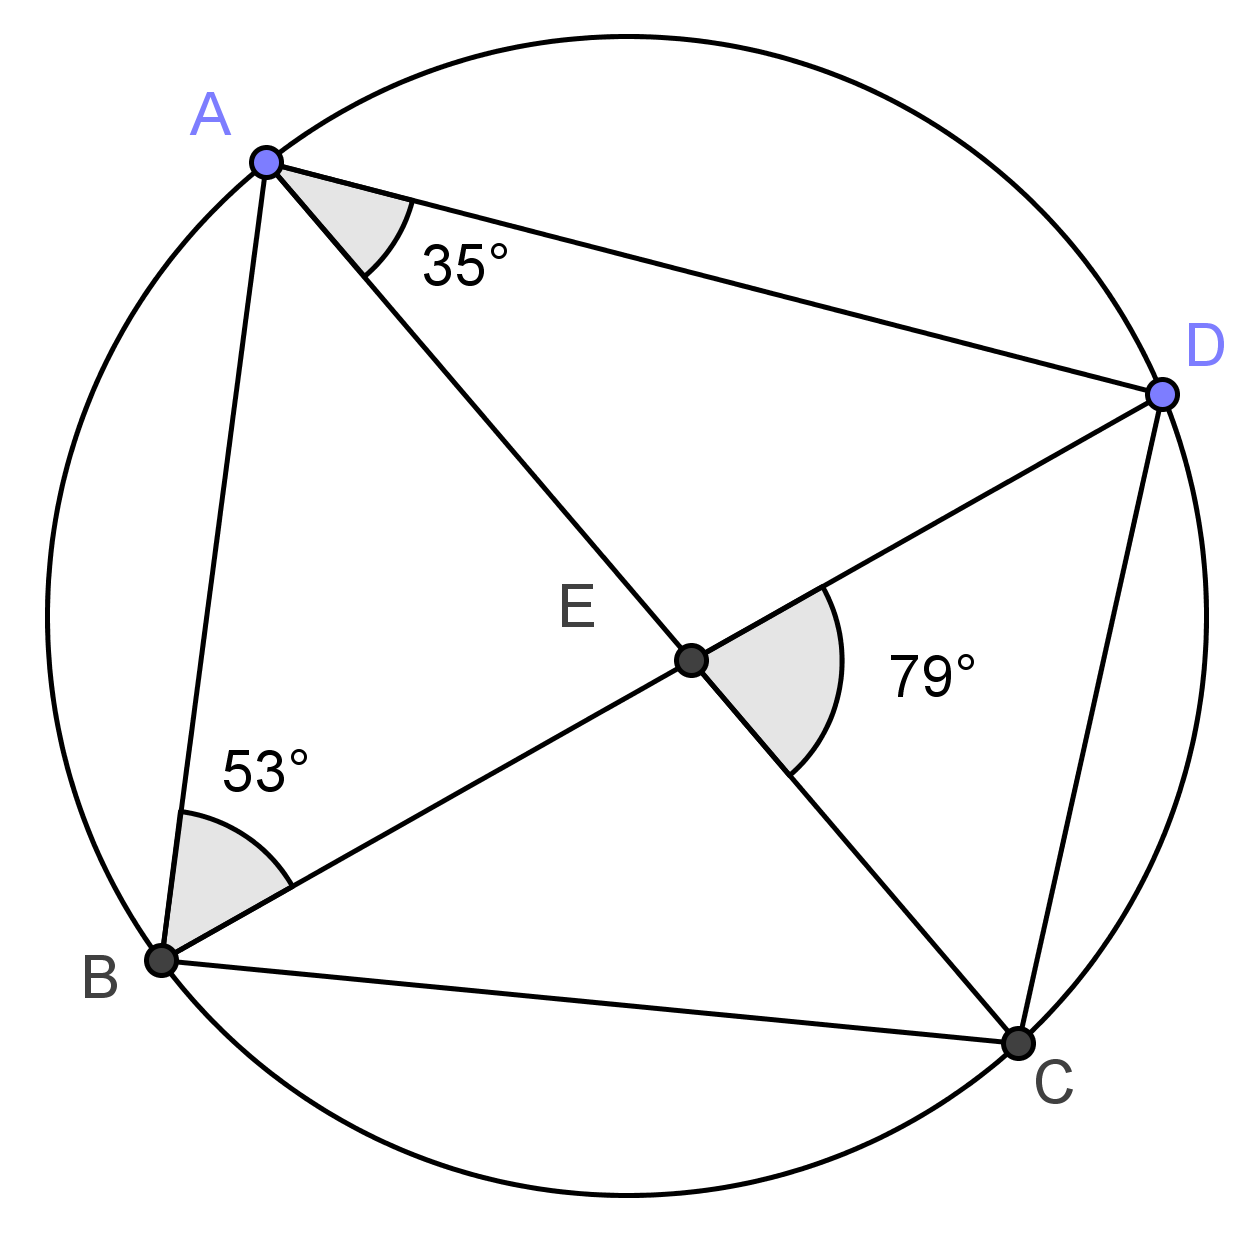
\includegraphics[width=5cm]{image/DS3.png}
\end{center}
\textit{Suggestion: Faire une figure � main lev�e sur votre copie.}
\end{document} 
